\documentclass[11pt,addpoints,answers]{exam}

%-----------------------------------------------------------------------------
% PACKAGES AND OTHER DOCUMENT CONFIGURATIONS
%-----------------------------------------------------------------------------

\usepackage[margin=1in]{geometry}
\usepackage{amsmath, amsfonts}
\usepackage{enumerate}
\usepackage{graphicx}
\usepackage{titling}
\usepackage{url}
\usepackage{xfrac}
\usepackage{natbib}
\usepackage{amssymb}
\usepackage{amsthm}
\usepackage{paralist}
\usepackage{epstopdf}
\usepackage{tabularx}
\usepackage{longtable}
\usepackage{multirow}
\usepackage{multicol}
\usepackage[colorlinks=true,urlcolor=blue]{hyperref}
\usepackage{algorithm}
\usepackage{algorithmicx}
\usepackage[noend]{algpseudocode}
\usepackage{float}
\usepackage{enumerate}
\usepackage{array}
\usepackage{environ}
\usepackage{times}
\usepackage{textcomp}
\usepackage{caption}
\usepackage{parskip} % For NIPS style paragraphs.
\usepackage[compact]{titlesec} % Less whitespace around titles
\usepackage[inline]{enumitem} % For inline enumerate* and itemize*
\usepackage{datetime}
\usepackage{comment}
% \usepackage{minted}
\usepackage{lastpage}
\usepackage{color}
\usepackage{xcolor}
\usepackage[final]{listings}
\usepackage{tikz}
\usetikzlibrary{shapes,decorations}
\usepackage{framed}
\usepackage{booktabs}
\usepackage{cprotect}
\usepackage{verbatim}
\usepackage{verbatimbox}
\usepackage{multicol}
\usepackage{hyperref}
\usepackage{subcaption}
\usepackage{mathtools} % For drcases
\usepackage{cancel}
\usepackage[many]{tcolorbox}
\usepackage{soul}
\usepackage[bottom]{footmisc}
\usepackage{bm}
\usepackage{wasysym}
\usepackage[utf8]{inputenc}
\usepackage{tikz}
\usetikzlibrary{arrows}
\usetikzlibrary{arrows.meta}
\usetikzlibrary{shapes.geometric}
\usetikzlibrary{positioning, arrows, automata, calc}
\usepackage{transparent}

\newtcolorbox[]{your_solution}[1][]{
    % breakable,
    enhanced,
    nobeforeafter,
    colback=white,
    title=Your Answer,
    sidebyside align=top,
    box align=top,
    #1
}

%%%%%%%%%%%%%%%%%%%%%%%%%%%%%%%%%%%%%%%%%%%
% Formatting for \CorrectChoice of "exam" %
%%%%%%%%%%%%%%%%%%%%%%%%%%%%%%%%%%%%%%%%%%%

\CorrectChoiceEmphasis{}
\checkedchar{\blackcircle}

%%%%%%%%%%%%%%%%%%%%%%%%%%%%%%%%%%%%%%%%%%%
% Rotated Column Headers                  %
%%%%%%%%%%%%%%%%%%%%%%%%%%%%%%%%%%%%%%%%%%%
\usepackage{adjustbox}
\usepackage{array}

%https://tex.stackexchange.com/questions/32683/rotated-column-titles-in-tabular

\newcolumntype{R}[2]{%
    >{\adjustbox{angle=#1,lap=\width-(#2)}\bgroup}%
    l%
    <{\egroup}%
}
\newcommand*\rot{\multicolumn{1}{R{45}{1em}}}% no optional argument here, please!

%%%%%%%%%%%%%%%%%%%%%%%%%%%%%%%%%%%%%%%%%%
% Custom commands                        %
%%%%%%%%%%%%%%%%%%%%%%%%%%%%%%%%%%%%%%%%%%

\newcommand{\vc}[1]{\boldsymbol{#1}}
\newcommand{\adj}[1]{\frac{d J}{d #1}}
\newcommand{\chain}[2]{\adj{#2} = \adj{#1}\frac{d #1}{d #2}}

\newcommand{\R}{\mathbb{R}}
\newcommand{\blackcircle}{\tikz\draw[black,fill=black] (0,0) circle (1ex);}
\renewcommand{\circle}{\tikz\draw[black] (0,0) circle (1ex);}

\newcommand{\emptysquare}{{\LARGE $\square$}\ \ }
\newcommand{\filledsquare}{{\LARGE $\blacksquare$}\ \ }
\newcommand{\emptycircle}{{\LARGE $\fullmoon$}\ \ }
\newcommand{\filledcircle}{{\LARGE $\newmoon$}\ \ }

\newcommand{\ntset}{test}

% mathcal
\newcommand{\Ac}{\mathcal{A}}
\newcommand{\Bc}{\mathcal{B}}
\newcommand{\Cc}{\mathcal{C}}
\newcommand{\Dc}{\mathcal{D}}
\newcommand{\Ec}{\mathcal{E}}
\newcommand{\Fc}{\mathcal{F}}
\newcommand{\Gc}{\mathcal{G}}
\newcommand{\Hc}{\mathcal{H}}
\newcommand{\Ic}{\mathcal{I}}
\newcommand{\Jc}{\mathcal{J}}
\newcommand{\Kc}{\mathcal{K}}
\newcommand{\Lc}{\mathcal{L}}
\newcommand{\Mc}{\mathcal{M}}
\newcommand{\Nc}{\mathcal{N}}
\newcommand{\Oc}{\mathcal{O}}
\newcommand{\Pc}{\mathcal{P}}
\newcommand{\Qc}{\mathcal{Q}}
\newcommand{\Rc}{\mathcal{R}}
\newcommand{\Sc}{\mathcal{S}}
\newcommand{\Tc}{\mathcal{T}}
\newcommand{\Uc}{\mathcal{U}}
\newcommand{\Vc}{\mathcal{V}}
\newcommand{\Wc}{\mathcal{W}}
\newcommand{\Xc}{\mathcal{X}}
\newcommand{\Yc}{\mathcal{Y}}
\newcommand{\Zc}{\mathcal{Z}}

% mathbb
\newcommand{\Ab}{\mathbb{A}}
\newcommand{\Bb}{\mathbb{B}}
\newcommand{\Cb}{\mathbb{C}}
\newcommand{\Db}{\mathbb{D}}
\newcommand{\Eb}{\mathbb{E}}
\newcommand{\Fb}{\mathbb{F}}
\newcommand{\Gb}{\mathbb{G}}
\newcommand{\Hb}{\mathbb{H}}
\newcommand{\Ib}{\mathbb{I}}
\newcommand{\Jb}{\mathbb{J}}
\newcommand{\Kb}{\mathbb{K}}
\newcommand{\Lb}{\mathbb{L}}
\newcommand{\Mb}{\mathbb{M}}
\newcommand{\Nb}{\mathbb{N}}
\newcommand{\Ob}{\mathbb{O}}
\newcommand{\Pb}{\mathbb{P}}
\newcommand{\Qb}{\mathbb{Q}}
\newcommand{\Rb}{\mathbb{R}}
\newcommand{\Sb}{\mathbb{S}}
\newcommand{\Tb}{\mathbb{T}}
\newcommand{\Ub}{\mathbb{U}}
\newcommand{\Vb}{\mathbb{V}}
\newcommand{\Wb}{\mathbb{W}}
\newcommand{\Xb}{\mathbb{X}}
\newcommand{\Yb}{\mathbb{Y}}
\newcommand{\Zb}{\mathbb{Z}}

% mathbf lowercase
\newcommand{\av}{\mathbf{a}}
\newcommand{\bv}{\mathbf{b}}
\newcommand{\cv}{\mathbf{c}}
\newcommand{\dv}{\mathbf{d}}
\newcommand{\ev}{\mathbf{e}}
\newcommand{\fv}{\mathbf{f}}
\newcommand{\gv}{\mathbf{g}}
\newcommand{\hv}{\mathbf{h}}
\newcommand{\iv}{\mathbf{i}}
\newcommand{\jv}{\mathbf{j}}
\newcommand{\kv}{\mathbf{k}}
\newcommand{\lv}{\mathbf{l}}
\newcommand{\mv}{\mathbf{m}}
\newcommand{\nv}{\mathbf{n}}
\newcommand{\ov}{\mathbf{o}}
\newcommand{\pv}{\mathbf{p}}
\newcommand{\qv}{\mathbf{q}}
\newcommand{\rv}{\mathbf{r}}
\newcommand{\sv}{\mathbf{s}}
\newcommand{\tv}{\mathbf{t}}
\newcommand{\uv}{\mathbf{u}}
\newcommand{\vv}{\mathbf{v}}
\newcommand{\wv}{\mathbf{w}}
\newcommand{\xv}{\mathbf{x}}
\newcommand{\yv}{\mathbf{y}}
\newcommand{\zv}{\mathbf{z}}

% mathbf uppercase
\newcommand{\Av}{\mathbf{A}}
\newcommand{\Bv}{\mathbf{B}}
\newcommand{\Cv}{\mathbf{C}}
\newcommand{\Dv}{\mathbf{D}}
\newcommand{\Ev}{\mathbf{E}}
\newcommand{\Fv}{\mathbf{F}}
\newcommand{\Gv}{\mathbf{G}}
\newcommand{\Hv}{\mathbf{H}}
\newcommand{\Iv}{\mathbf{I}}
\newcommand{\Jv}{\mathbf{J}}
\newcommand{\Kv}{\mathbf{K}}
\newcommand{\Lv}{\mathbf{L}}
\newcommand{\Mv}{\mathbf{M}}
\newcommand{\Nv}{\mathbf{N}}
\newcommand{\Ov}{\mathbf{O}}
\newcommand{\Pv}{\mathbf{P}}
\newcommand{\Qv}{\mathbf{Q}}
\newcommand{\Rv}{\mathbf{R}}
\newcommand{\Sv}{\mathbf{S}}
\newcommand{\Tv}{\mathbf{T}}
\newcommand{\Uv}{\mathbf{U}}
\newcommand{\Vv}{\mathbf{V}}
\newcommand{\Wv}{\mathbf{W}}
\newcommand{\Xv}{\mathbf{X}}
\newcommand{\Yv}{\mathbf{Y}}
\newcommand{\Zv}{\mathbf{Z}}

% bold greek lowercase
\newcommand{\alphav     }{\boldsymbol \alpha     }
\newcommand{\betav      }{\boldsymbol \beta      }
\newcommand{\gammav     }{\boldsymbol \gamma     }
\newcommand{\deltav     }{\boldsymbol \delta     }
\newcommand{\epsilonv   }{\boldsymbol \epsilon   }
\newcommand{\varepsilonv}{\boldsymbol \varepsilon}
\newcommand{\zetav      }{\boldsymbol \zeta      }
\newcommand{\etav       }{\boldsymbol \eta       }
\newcommand{\thetav     }{\boldsymbol \theta     }
\newcommand{\varthetav  }{\boldsymbol \vartheta  }
\newcommand{\iotav      }{\boldsymbol \iota      }
\newcommand{\kappav     }{\boldsymbol \kappa     }
\newcommand{\varkappav  }{\boldsymbol \varkappa  }
\newcommand{\lambdav    }{\boldsymbol \lambda    }
\newcommand{\muv        }{\boldsymbol \mu        }
\newcommand{\nuv        }{\boldsymbol \nu        }
\newcommand{\xiv        }{\boldsymbol \xi        }
\newcommand{\omicronv   }{\boldsymbol \omicron   }
\newcommand{\piv        }{\boldsymbol \pi        }
\newcommand{\varpiv     }{\boldsymbol \varpi     }
\newcommand{\rhov       }{\boldsymbol \rho       }
\newcommand{\varrhov    }{\boldsymbol \varrho    }
\newcommand{\sigmav     }{\boldsymbol \sigma     }
\newcommand{\varsigmav  }{\boldsymbol \varsigma  }
\newcommand{\tauv       }{\boldsymbol \tau       }
\newcommand{\upsilonv   }{\boldsymbol \upsilon   }
\newcommand{\phiv       }{\boldsymbol \phi       }
\newcommand{\varphiv    }{\boldsymbol \varphi    }
\newcommand{\chiv       }{\boldsymbol \chi       }
\newcommand{\psiv       }{\boldsymbol \psi       }
\newcommand{\omegav     }{\boldsymbol \omega     }

% bold greek uppercase
\newcommand{\Gammav     }{\boldsymbol \Gamma     }
\newcommand{\Deltav     }{\boldsymbol \Delta     }
\newcommand{\Thetav     }{\boldsymbol \Theta     }
\newcommand{\Lambdav    }{\boldsymbol \Lambda    }
\newcommand{\Xiv        }{\boldsymbol \Xi        }
\newcommand{\Piv        }{\boldsymbol \Pi        }
\newcommand{\Sigmav     }{\boldsymbol \Sigma     }
\newcommand{\Upsilonv   }{\boldsymbol \Upsilon   }
\newcommand{\Phiv       }{\boldsymbol \Phi       }
\newcommand{\Psiv       }{\boldsymbol \Psi       }
\newcommand{\Omegav     }{\boldsymbol \Omega     }

%%%%%%%%%%%%%%%%%%%%%%%%%%%%%%%%%%%%%%%%%%%
% Code highlighting with listings         %
%%%%%%%%%%%%%%%%%%%%%%%%%%%%%%%%%%%%%%%%%%%

\definecolor{bluekeywords}{rgb}{0.13,0.13,1}
\definecolor{greencomments}{rgb}{0,0.5,0}
\definecolor{redstrings}{rgb}{0.9,0,0}
\definecolor{light-gray}{gray}{0.95}

\newcommand{\MYhref}[3][blue]{\href{#2}{\color{#1}{#3}}}%

\definecolor{dkgreen}{rgb}{0,0.6,0}
\definecolor{gray}{rgb}{0.5,0.5,0.5}
\definecolor{mauve}{rgb}{0.58,0,0.82}

\lstdefinelanguage{Shell}{
  keywords={tar, cd, make},
  %keywordstyle=\color{bluekeywords}\bfseries,
  alsoletter={+},
  ndkeywords={python3, python, py, javac, java, gcc, c, g++, cpp, .txt, octave, m, .tar},
  %ndkeywordstyle=\color{bluekeywords}\bfseries,
  identifierstyle=\color{black},
  sensitive=false,
  comment=[l]{//},
  morecomment=[s]{/*}{*/},
  commentstyle=\color{purple}\ttfamily,
  %stringstyle=\color{red}\ttfamily,
  morestring=[b]',
  morestring=[b]",
  backgroundcolor = \color{light-gray}
}

\lstset{columns=fixed, basicstyle=\ttfamily,
    backgroundcolor=\color{light-gray},xleftmargin=0.5cm,frame=tlbr,framesep=4pt,framerule=0pt}


%%%%%%%%%%%%%%%%%%%%%%%%%%%%%%%%%%%%%%%%%%%
% Custom box for highlights               %
%%%%%%%%%%%%%%%%%%%%%%%%%%%%%%%%%%%%%%%%%%%

% Define box and box title style
\tikzstyle{mybox} = [fill=blue!10, very thick,
    rectangle, rounded corners, inner sep=1em, inner ysep=1em]

\NewEnviron{notebox}{
\resizebox{1.02\textwidth}{!}{%

\begin{tikzpicture}
\node [mybox] (box){
    \begin{minipage}{\textwidth}
        \BODY
    \end{minipage}
};
\end{tikzpicture}
}%
}

%%%%%%%%%%%%%%%%%%%%%%%%%%%%%%%%%%%%%%%%%%%
% Commands showing / hiding solutions     %
%%%%%%%%%%%%%%%%%%%%%%%%%%%%%%%%%%%%%%%%%%%

%% To HIDE SOLUTIONS (to post at the website for students), set this value to 0:
\def\issoln{0}
% Some commands to allow solutions to be embedded in the assignment file.
\ifcsname issoln\endcsname \else \def\issoln{1} \fi
% Default to an empty solutions environ.
\NewEnviron{soln}{}{}
\if\issoln 1
%Otherwise, include solutions as below.
\RenewEnviron{soln}{
    \leavevmode\color{red}\ignorespaces
    \textbf{Solution} \BODY
    % \BODY
}{}
\fi

%% qauthor environment:
% Default to an empty qauthor environ.
\NewEnviron{qauthor}{}{}
%% To HIDE TAGS set this value to 0:
\def\showtags{0}
%%%%%%%%%%%%%%%%
\ifcsname showtags\endcsname \else \def\showtags{1} \fi
% Default to an empty tags environ.
\NewEnviron{tags}{}{}
\if\showtags 1
% Otherwise, include solutions as below.
\RenewEnviron{tags}{
    \fbox{
    \leavevmode\color{blue}\ignorespaces
    \textbf{TAGS:} \texttt{\url{\BODY}}
    }
    \vspace{-.5em}
}{}
\fi

%%%%%%%%%%%%%%%%%%%%%%%%%%%%%%%%%%%%%%%%%%%
% Commands for customizing the assignment %
%%%%%%%%%%%%%%%%%%%%%%%%%%%%%%%%%%%%%%%%%%%

\newcommand{\courseNum}{10-301/10-601}
\newcommand{\courseName}{ Introduction to Machine Learning }
\newcommand{\courseSem}{Spring 2023}
\newcommand{\courseUrl}{\url{http://www.cs.cmu.edu/~mgormley/courses/10601/}}
\newcommand{\hwNum}{Homework 4}
\newcommand{\hwTopic}{Logistic Regression}
\newcommand{\hwName}{\hwNum: \hwTopic}
\newcommand{\dueDate}{Sunday, Feb 26 at 11:59 PM}

\lhead{\hwName}
\rhead{\courseNum}
\cfoot{\thepage{} of \numpages{}}


\title{\textsc{\hwNum}: \textsc{\hwTopic}
%\thanks{Compiled on \today{} at \currenttime{}}
} % Title


\author{\courseNum \courseName (\courseSem)\\
\url{http://www.cs.cmu.edu/~mgormley/courses/10601/} \\
OUT: Friday, Feb 17 \\
DUE: \dueDate{} \\
TAs: Alex, Emaan, Markov, Neural, Pranay, Pranit, Tanvi
}

\newcommand{\homeworktype}{\string written/programming}

\date{}


%%%%%%%%%%%%%%%%%%%%%%%%%%%%%%%%%%%%%%%%%%%%%%%%%
% Useful commands for typesetting the questions %
%%%%%%%%%%%%%%%%%%%%%%%%%%%%%%%%%%%%%%%%%%%%%%%%%

\newcommand \expect {\mathbb{E}}
\newcommand \mle [1]{{\hat #1}^{\rm MLE}}
\newcommand \map [1]{{\hat #1}^{\rm MAP}}
\newcommand \argmax {\operatorname*{argmax}}
\newcommand \argmin {\operatorname*{argmin}}
\newcommand \code [1]{{\tt #1}}
\newcommand \datacount [1]{\#\{#1\}}
\newcommand \ind [1]{\mathbb{I}\{#1\}}

%%%%%%%%%%%%%%%%%%%%%%%%%%
% Document configuration %
%%%%%%%%%%%%%%%%%%%%%%%%%%

% Don't display a date in the title and remove the white space
\predate{}
\postdate{}
\date{}

% Don't display an author and remove the white space
%\preauthor{}
%\postauthor{}

% Solo and group questions
\newcommand{\solo}{\textbf{[SOLO]} }
\newcommand{\group}{\textbf{[GROUP]} }

% Question type commands
\newcommand{\sall}{\textbf{Select all that apply: }}
\newcommand{\sone}{\textbf{Select one: }}
\newcommand{\tf}{\textbf{True or False: }}

% AdaBoost commands
\newcommand{\trainerr}[1]{\hat{\epsilon}_S \left(#1\right)}
\newcommand{\generr}[1]{\epsilon \left(#1\right)}
\newcommand{\D}{\mathcal{D}}
\newcommand{\margin}{\text{margin}}
\newcommand{\sign}{\text{sign}}
\newcommand{\PrS}{\hat{\Pr_{(x_i, y_i) \sim S}}}
\newcommand{\PrSinline}{\hat{\Pr}_{(x_i, y_i) \sim S}}  % inline PrS

% Abhi messing around with examdoc
\qformat{\textbf{{\Large \thequestion \; \; \thequestiontitle \ (\totalpoints \ points)}} \hfill}
\renewcommand{\thequestion}{\arabic{question}}
\renewcommand{\questionlabel}{\thequestion.}

\renewcommand{\thepartno}{\arabic{partno}}
\renewcommand{\partlabel}{\thepartno.}
\renewcommand{\partshook}{\setlength{\leftmargin}{0pt}}

\renewcommand{\thesubpart}{\alph{subpart}}
\renewcommand{\subpartlabel}{(\thesubpart)}

\renewcommand{\thesubsubpart}{\roman{subsubpart}}
\renewcommand{\subsubpartlabel}{\thesubsubpart.}

% copied from stack overflow, as all good things are
\newcommand\invisiblesection[1]{%
  \refstepcounter{section}%
  \addcontentsline{toc}{section}{\protect\numberline{\thesection}#1}%
  \sectionmark{#1}}

% quite possibly the worst workaround i have made for this class
\newcommand{\sectionquestion}[1]{
\titledquestion{#1}
\invisiblesection{#1}
~\vspace{-1em}
}

%%%%%%%%%%%%%%%%%%%%%%%%%%%%%%%%%%%%%%%%%%%
% New Environment for Pseudocode          %
%%%%%%%%%%%%%%%%%%%%%%%%%%%%%%%%%%%%%%%%%%%

% Python style for highlighting
\DeclareFixedFont{\ttb}{T1}{txtt}{bx}{n}{10} % for bold
\DeclareFixedFont{\ttm}{T1}{txtt}{m}{n}{10}  % for normal

\definecolor{deepblue}{rgb}{0,0,0.5}
\definecolor{deepred}{rgb}{0.6,0,0}
\definecolor{deepgreen}{rgb}{0,0.5,0}

\newcommand\pythonstyle{\lstset{
language=Python,
basicstyle=\ttm,
morekeywords={self},              % Add keywords here
keywordstyle=\ttb\color{deepblue},
emphstyle=\ttb\color{deepred},    % Custom highlighting style
stringstyle=\color{deepgreen},
frame=tb,                         % Any extra options here
showstringspaces=false,
xleftmargin=0pt
}}


% Python environment
\lstnewenvironment{your_code_solution}[1][]
{
\pythonstyle
\lstset{#1}
}
{}


%%%%%%%%%%%%%%%%%%
% Begin Document %
%%%%%%%%%%%%%%%%%%
\begin{document}

\maketitle



\begin{notebox}
\paragraph{Summary} In this assignment, you will build a sentiment polarity analyzer, which will be capable of analyzing the overall sentiment polarity (positive or negative) for restaurant reviews using logistic regression. In the written component, you will study linear and logistic regression.
\end{notebox}
\newcommand \maxsubs {10 }
\section*{START HERE: Instructions}
\begin{itemize}

\item \textbf{Collaboration Policy}: Please read the collaboration policy here: \url{http://www.cs.cmu.edu/~mgormley/courses/10601/syllabus.html}

\item\textbf{Late Submission Policy:} See the late submission policy here: \url{http://www.cs.cmu.edu/~mgormley/courses/10601/syllabus.html}

\item\textbf{Submitting your work:} You will use Gradescope to submit
  answers to all questions\ifthenelse{\equal{\homeworktype}{\string written}}{}{ and code}. Please
  follow instructions at the end of this PDF to correctly submit all your code to Gradescope.

  \begin{itemize}
    
 % COMMENT IF NOT USING CANVAS
\begin{comment}
  \item \textbf{Canvas:} Canvas (\url{https://canvas.cmu.edu}) will be
    used for quiz-style problems (e.g. multiple choice, true / false,
    numerical answers). Grading is done automatically.
    %
    You may only \textbf{submit once} on canvas, so be sure of your
    answers before you submit. However, canvas allows you to work on
    your answers and then close out of the page and it will save your
    progress.  You will not be granted additional submissions, so
    please be confident of your solutions when you are submitting your
    assignment.
    %
    {\color{red} The above is true for future assignments, but this one
    allows {\bf unlimited submissions}.}
\end{comment}
    
  % COMMENT IF NOT USING GRADESCOPE
   \item \textbf{Written:} For written problems such as short answer, multiple choice, derivations, proofs, or plots, please use the provided template. Submissions can be handwritten onto the template, but should be labeled and clearly legible. If your writing is not legible, you will not be awarded marks. Alternatively, submissions can be written in \LaTeX{}. Each derivation/proof should be completed in the boxes provided. You are responsible for ensuring that your submission contains exactly the same number of pages and the same alignment as our PDF template. If you do not follow the template, your assignment may not be graded correctly by our AI assisted grader and there will be a \textbf{\textcolor{red}{2\% penalty}} (e.g., if the homework is out of 100 points, 5 points will be deducted from your final score).

  %   COMMENT IF NOT USING GRADESCOPE AUTOGRADER
  \ifthenelse{\equal{\homeworktype}{\string written}}{}{
\item \textbf{Programming:} You will submit your code for programming questions on the homework to Gradescope (\url{https://gradescope.com}). After uploading your code, our grading scripts will autograde your assignment by running your program on a virtual machine (VM). When you are developing, check that the version number of the programming language environment (e.g. Python 3.9.12) and versions of permitted libraries (e.g.  \texttt{numpy} 1.23.0) match those used on Gradescope. You have \maxsubs free Gradescope programming submissions. After \maxsubs submissions, you will begin to lose points from your total programming score. We recommend debugging your implementation on your local machine (or the Linux servers) and making sure your code is running correctly first before submitting your code to Gradescope.}

  \end{itemize}
  
\ifthenelse{\equal{\homeworktype}{\string written}}{}{\item\textbf{Materials:} The data and reference output that you will need in order to complete this assignment is posted along with the writeup and template on the course website.}

\end{itemize}


%\ifthenelse{\equal{\homeworktype}{\string written}}{}{\begin{notebox}
%\paragraph{Linear Algebra Libraries} When implementing machine learning algorithms, it is often convenient to have a linear algebra library at your disposal. In this assignment, Java users may use EJML\footnote{\url{https://ejml.org}} or ND4J\footnote{\url{https://javadoc.io/doc/org.nd4j/nd4j-api/latest/index.html}} and C++ users may use Eigen\footnote{\url{http://eigen.tuxfamily.org/}}. Details below. 
%
%(As usual, Python users have NumPy.)
%
%\begin{description}
%\item[EJML for Java] EJML is a pure Java linear algebra package with three interfaces. We strongly recommend using the SimpleMatrix interface. The autograder will use EJML version 0.41. When compiling and running your code, we will add the additional command line argument {\footnotesize{\lstinline{-cp "linalg_lib/ejml-v0.41-libs/*:linalg_lib/nd4j-v1.0.0-M1.1-libs/*:./"}}}
%to ensure that all the EJML jars are on the classpath as well as your code. 

%\item[ND4J for Java] ND4J is a library for multidimensional tensors with an interface akin to Python's NumPy. The autograder will use ND4J version 1.0.0-M1.1. When compiling and running your code, we will add the additional command line argument {\footnotesize{\lstinline{-cp "linalg_lib/ejml-v0.41-libs/*:linalg_lib/nd4j-v1.0.0-M1.1-libs/*:./"}}} to ensure that all the ND4J jars are on the classpath as well as your code. 

%\item[Eigen for C++] Eigen is a header-only library, so there is no linking to worry about---just \lstinline{#include} whatever components you need. The autograder will use Eigen version 3.4.0. The command line arguments above demonstrate how we will call you code. When compiling your code we will include, the argument \lstinline{-I./linalg_lib} in order to include the \lstinline{linalg_lib/Eigen} subdirectory, which contains all the headers.

%\end{description} 
%We have included the correct versions of EJML/ND4J/Eigen in the \lstinline{linalg_lib.zip} posted on the Coursework page of the course website for your convenience. It contains the same \lstinline{linalg_lib/} directory that we will include in the current working directory when running your tests. Do {\bf not} include EJML, ND4J, or Eigen in your homework submission; the autograder will ensure that they are in place. 
%\end{notebox}}\clearpage

\section*{Instructions for Specific Problem Types}

For ``Select One" questions, please fill in the appropriate bubble completely:

\begin{quote}
\textbf{Select One:} Who taught this course?
    \begin{checkboxes}
     \CorrectChoice Matt Gormley
     \choice Marie Curie
     \choice Noam Chomsky
    \end{checkboxes}
\end{quote}

If you need to change your answer, you may cross out the previous answer and bubble in the new answer:

\begin{quote}
\textbf{Select One:} Who taught this course?
    {
    \begin{checkboxes}
     \CorrectChoice Henry Chai
     \choice Marie Curie \checkboxchar{\xcancel{\blackcircle}{}}
     \choice Noam Chomsky
    \end{checkboxes}
    }
\end{quote}

For ``Select all that apply" questions, please fill in all appropriate squares completely:

\begin{quote}
\textbf{Select all that apply:} Which are scientists?
    {%
    \checkboxchar{$\Box$} \checkedchar{$\blacksquare$} % change checkbox style locally
    \begin{checkboxes}
    \CorrectChoice Stephen Hawking 
    \CorrectChoice Albert Einstein
    \CorrectChoice Isaac Newton
    \choice I don't know
    \end{checkboxes}
    }
\end{quote}

Again, if you need to change your answer, you may cross out the previous answer(s) and bubble in the new answer(s):

\begin{quote}
\textbf{Select all that apply:} Which are scientists?
    {%
    \checkboxchar{\xcancel{$\blacksquare$}} \checkedchar{$\blacksquare$} % change checkbox style locally
    \begin{checkboxes}
    \CorrectChoice Stephen Hawking 
    \CorrectChoice Albert Einstein
    \CorrectChoice Isaac Newton
    \choice I don't know
    \end{checkboxes}
    }
\end{quote}

For questions where you must fill in a blank, please make sure your final answer is fully included in the given space. You may cross out answers or parts of answers, but the final answer must still be within the given space.

\begin{quote}
\textbf{Fill in the blank:} What is the course number?

\begin{tcolorbox}[fit,height=1cm, width=4cm, blank, borderline={1pt}{-2pt},nobeforeafter]
    \begin{center}\huge10-601\end{center}
    \end{tcolorbox}\hspace{2cm}
    \begin{tcolorbox}[fit,height=1cm, width=4cm, blank, borderline={1pt}{-2pt},nobeforeafter]
    \begin{center}\huge10-\xcancel{6}301\end{center}
    \end{tcolorbox}
\end{quote}

\clearpage

{\LARGE \bf Written Questions (\numpoints \ points)}

\begin{questions}
\sectionquestion{\LaTeX{} Bonus Point and Template Alignment}
\begin{parts}
    \part[1] \sone Did you use \LaTeX{} for the entire written portion of this homework?
    
    \begin{checkboxes}
        % YOUR ANSWER
        % Change \choice to \CorrectChoice for the appropriate selection/selections 
        \CorrectChoice Yes 
        \choice No
    \end{checkboxes}

    \part[0] \sone I have ensured that my final submission is aligned with the original template given to me in the handout file and that I haven't deleted or resized any items or made any other modifications which will result in a misaligned template. I understand that incorrectly responding yes to this question will result in a penalty equivalent to 2\% of the points on this assignment.\\
    \textbf{Note:} Failing to answer this question will not exempt you from the 2\% misalignment penalty.
    
    \begin{checkboxes}
        % YOUR ANSWER
        % Change \choice to \CorrectChoice for the appropriate selection/selections 
        \CorrectChoice Yes 
    \end{checkboxes}
\end{parts}
\vspace*{1.2cm}

\sectionquestion{Linear Regression} 
\begin{parts}
\part We would like to fit a linear regression model to the dataset 
$$
\Dc = \left\{\left(\xv^{(1)},y^{(1)}\right), \left(\xv^{(2)},y^{(2)}\right),\cdots, \left(\xv^{(N)},y^{(N)}\right)\right\}
$$ with $\xv^{(i)} \in \mathbb{R}^M$ by minimizing the ordinary least square (OLS) objective function:
$$
J(\wv) = \frac{1}{2}\sum_{i=1}^N\left(y^{(i)} - \sum_{j=1}^M w_j x_j^{(i)}\right)^2.
$$
\begin{subparts}
    \subpart[2] \sone
    We solve for each coefficient $w_k$ ($1\leq k\leq M$) by deriving an expression of $w_k$ from the critical point $\frac{\partial J(\wv)}{\partial w_k} = 0$. What is the expression for each $w_k$ in terms of the dataset 
    $(\xv^{(1)},y^{(1)})$, $\cdots$, $(\xv^{(N)},y^{(N)})$ and $w_1,\cdots,w_{k-1},w_{k+1},\cdots,w_M$?

    \begin{checkboxes}
        % YOUR ANSWER
        % Change \choice to \CorrectChoice for the appropriate selection/selections 
        \CorrectChoice $w_k = \frac{\sum_{i=1}^N x_k^{(i)}(y^{(i)}-\sum_{j=1,j\neq k}^M w_j x_j^{(i)})}{\sum_{i=1}^N (x_k^{(i)})^2}$
        \choice $w_k = \frac{\sum_{i=1}^N x_k^{(i)}(y^{(i)}-\sum_{j=1,j\neq k}^M w_j x_j^{(i)})}{\sum_{i=1}^N (y^{(i)})^2}$
        \choice $w_k = \frac{\sum_{i=1}^N x_k^{(i)}(y^{(i)}-\sum_{j=1,j\neq k}^M w_j x_j^{(i)})}{\sum_{i=1}^N (x_k^{(i)} y^{(i)})^2}$
        \choice $w_k = \sum_{i=1}^N x_k^{(i)}(y^{(i)}-\sum_{j=1}^M w_j x_j^{(i)})$
    \end{checkboxes}


\vspace*{7mm}
    
    \subpart[1] \sone How many coefficients ($w_k$) do you need to estimate? When solving for these coefficients, how many equations do you have?

    \begin{checkboxes}
        % YOUR ANSWER
        % Change \choice to \CorrectChoice for the appropriate selection/selections 
        \CorrectChoice $M$ coefficients, $M$ equations
        \choice $M$ coefficients, $N$ equations
        \choice $N$ coefficients, $M$ equations
        \choice $N$ coefficients, $N$ equations
    \end{checkboxes}
    
\end{subparts}

\clearpage
\part[1] Consider a dataset $D$ such that we fit a line $y = w_1 x + b_1$. Let $\Bar{x}$ and $\Bar{y}$ be the mean of the $x$ and $y$ coordinates, respectively. After mean centering the dataset to create $D_{new} =\big((x^{(1)} - \Bar{x}, y^{(1)} - \Bar{y}), \ldots, (x^{(n)} - \Bar{x}, y^{(n)} - \Bar{y}) \big)$, let the solution to linear regression on $D_{new}$ be $y = w_2 x + b_2$. Explain how $w_2$ compares to $w_1$ and justify.

    \begin{checkboxes}
        % YOUR ANSWER
        % Change \choice to \CorrectChoice for the appropriate selection/selections 
        \choice $w_2 > w_1$. Mean centering lowers the value of the bias term, which increases the slope of the regression line.
        \choice $w_2 < w_1$. Mean centering decreases the variance of the data, so the regression line will not be as steep.
        \CorrectChoice $w_2 = w_1$. Mean centering data shifts the data and does not scale the coordinates; therefore, it does not change the fitted regression line's slope.
        \choice Not enough information to decide. Mean centering can either increase or decrease our label values, so it may make our regression line either more or less steep.
    \end{checkboxes}


    \end{parts}
    \newpage

\sectionquestion{Logistic Regression: Warm-Up}
\label{sec:warm-up}

The following questions should be completed before you start the programming component of this assignment.

The following dataset consists of 4 training examples, where $x_k^{(i)}$ denotes the $k$-th dimension of the $i$-th training example $\xv^{(i)}$, and $y^{(i)}$ is the corresponding label ($k \in \{1, 2, 3\}$ and $i \in \{1, 2, 3, 4\}$).

\begin{center}
\begin{tabular}{|c|c|c|c|c|c|c|}
\hline
$i$ & $x_{1}$ & $x_{2}$ & $x_{3}$ & $y$ \\ \hline
1   & 0       &       0 &       1 & 0   \\ \hline
2   & 0       &       1 &       0 & 1   \\ \hline
3   & 0       &       1 &       1 & 1   \\ \hline
4   & 1       &       0 &       0 & 0   \\ \hline

\end{tabular}
\end{center}

A binary logistic regression model is trained on this dataset, and the parameter vector $\thetav$ after training is

\[\thetav = \begin{bmatrix}1.5 & 2 & 1\end{bmatrix}^T.\]

\textit{Note}: There is \textbf{no intercept term} used in this problem.

Use the data above to answer the following questions. For all numerical answers, please use one number rounded to the fourth decimal place; e.g., 0.1234. Showing your work in these questions is optional, but it is recommended to help us understand where any misconceptions may occur.

\begin{parts}
    \part[2] Calculate  $J(\thetav$), $\frac{1}{N}$ times the negative log-likelihood over the given data and parameter $\thetav$. (Note here we are using natural log, i.e., the base is $e$). 
    
    \begin{your_solution}[title=$J(\thetav)$,height=2cm,width=3cm]
    % YOUR ANSWER
    0.3464
    \end{your_solution}
    
    \begin{your_solution}[title=Work,height=8cm]
    % YOUR ANSWER
    \end{your_solution}
    
    \pagebreak
    
    \part[2] Calculate the gradients $\frac{\partial J(\thetav)}{\partial \theta_j}$ with respect to $\theta_{j}$ for all $j \in \{1, 2, 3\}$.

    \begin{your_solution}[title=$\partial J(\thetav)/\partial \theta_1$,height=1.8cm,width=5.2cm]
    % YOUR ANSWER 
    0.2044
    \end{your_solution}
    \begin{your_solution}[title=$\partial J(\thetav)/\partial \theta_2$,height=1.8cm,width=5.2cm]
    % YOUR ANSWER 
    -0.4165
    \end{your_solution}
    \begin{your_solution}[title=$\partial J(\thetav)/\partial \theta_3$,height=1.8cm,width=5.2cm]
    % YOUR ANSWER 
    0.1709
    \end{your_solution}
    
    \begin{your_solution}[title=Work,height=18cm]
    % YOUR ANSWER
    \end{your_solution}

    
    \clearpage
    
    \part[1] Update the parameters following the parameter update step $\theta_j \leftarrow \theta_j - \eta \frac{\partial J(\thetav)}{\partial \theta_j}$ and write the updated (numerical) value of the vector $\thetav$. Use learning rate $\eta = 1$.

    \begin{your_solution}[title=$\theta_1$,height=1.8cm,width=5.2cm]
    % YOUR ANSWER
    1.2956 
    \end{your_solution}
    \begin{your_solution}[title=$\theta_2$,height=1.8cm,width=5.2cm]
    % YOUR ANSWER 
    2.4165
    \end{your_solution}
    \begin{your_solution}[title=$\theta_3$,height=1.8cm,width=5.2cm]
    % YOUR ANSWER 
    0.8291
    \end{your_solution}
    
    \begin{your_solution}[title=Work, height=6cm]
    % YOUR ANSWER 
    \end{your_solution}
    
    \clearpage
    
    


\clearpage
 
\end{parts}

\sectionquestion{Logistic Regression: Analysis}

\begin{parts}
        
    \part[2] \sall Which of the following are true about logistic regression?
    
    {%
    \checkboxchar{$\Box$} \checkedchar{$\blacksquare$}
    \begin{checkboxes}
        \CorrectChoice Our formulation of binary logistic regression will work with both continuous and binary features.
        \CorrectChoice Binary Logistic Regression will form a linear decision boundary in our feature space, assuming no feature engineering.
        \choice The sigmoid function is convex.
        \choice The negative log-likelihood function for logistic regression is not convex so gradient descent may get stuck in a sub-optimal local minimum.
        \choice None of the above.
    \end{checkboxes}
    }
    
    
    
    \vspace*{1.2cm}
    
    \part[1] \sone The \emph{average} negative log-likelihood $J(\thetav)$ for binary logistic regression can be expressed as 
    $$J(\thetav) = \frac{1}{N}\sum_{i=1}^N  \left[-y^{(i)}\left(\thetav^T\xv^{\left(i\right)}\right)+\log\left(1+\exp(\thetav^T\xv^{\left(i\right)})\right)\right]$$
    where $\xv^{(i)}\in \mathbb{R}^{M+1}$ is the column vector of the feature values of the $i$-th data point, $y^{(i)}\in\{0, 1\}$ is the $i$-th class label, $\thetav\in\mathbb{R}^{M+1}$ is the weight vector. When we want to perform logistic ridge regression (i.e. with $\ell_2$ regularization), we modify our objective function to be 
    $$ f(\thetav) = J(\thetav) + \lambda \frac{1}{2}\sum_{j=0}^M \theta_j^2$$
    where $\lambda$ is the regularization weight, $\theta_j$ is the $j$th element in the weight vector $\thetav$. Suppose we are updating $\theta_k$ with learning rate $\eta$, which of the following is the correct expression for the update?
    
    \begin{checkboxes}
        % YOUR ANSWER
        \choice 
            $\theta_k\leftarrow \theta_k + \eta \frac{\partial f(\thetav)}{\partial \theta_k}$ where 
            $ \frac{\partial f(\thetav)}{\partial \theta_k}=\frac{1}{N}\sum_{i=1}^N \left[x^{(i)}_k\left(y^{(i)} -\frac{\exp(\thetav^T \xv^{(i)})}{1+\exp(\thetav^T \xv^{(i)})} \right)\right]+\lambda \theta_k$
        \choice 
            $\theta_k\leftarrow \theta_k + \eta \frac{\partial f(\thetav)}{\partial \theta_k}$ where 
            $ \frac{\partial f(\thetav)}{\partial \theta_k}=\frac{1}{N}\sum_{i=1}^N \left[x^{(i)}_k\left(-y^{(i)} +\frac{\exp(\thetav^T \xv^{(i)})}{1+\exp(\thetav^T \xv^{(i)})} \right)\right]-\lambda \theta_k$
        \CorrectChoice 
            $\theta_k\leftarrow \theta_k - \eta \frac{\partial f(\thetav)}{\partial \theta_k}$ where 
            $ \frac{\partial f(\thetav)}{\partial \theta_k}=\frac{1}{N}\sum_{i=1}^N \left[x^{(i)}_k\left(-y^{(i)} +\frac{\exp(\thetav^T \xv^{(i)})}{1+\exp(\thetav^T \xv^{(i)})} \right)\right]+\lambda \theta_k$
        \choice
            $\theta_k\leftarrow \theta_k - \eta \frac{\partial f(\thetav)}{\partial \theta_k}$ where 
            $ \frac{\partial f(\thetav)}{\partial \theta_k}=\frac{1}{N}\sum_{i=1}^N \left[x^{(i)}_k\left(-y^{(i)} -\frac{\exp(\thetav^T \xv^{(i)})}{1+\exp(\thetav^T \xv^{(i)})} \right)\right]+\lambda \theta_k$
    \end{checkboxes}

    
    \newpage
    \part[2] Data is separable in one dimension if there exists a threshold $t$ such that all values less than $t$ have one class label and all values greater than or equal to $t$ have the other class label.
    If you train an unregularized logistic regression model for infinite iterations on training data that is separable in at least one dimension,
    the corresponding weight(s) can go to infinity in magnitude.
    What is an explanation for this phenomenon? \\
    \textit{Hint}: Think about what happens to the probabilities if we train an unregularized logistic regression model, and the role of the weights when calculating such probabilities.

    
    \begin{your_solution}[height=6cm]
    % YOUR ANSWER 
    \end{your_solution}
    
    \part[2] \sall How does regularization (such as $\ell_1$ and $\ell_2$) help correct the problem in the previous question?

    {%
    \checkboxchar{$\Box$} \checkedchar{$\blacksquare$}
    \begin{checkboxes}
        \choice $\ell_1$ regularization prevents weights from going to infinity by penalizing the count of non-zero weights.
        \CorrectChoice $\ell_1$ regularization prevents weights from going to infinity by reducing some of the weights to 0, effectively removing some of the features. 
        \CorrectChoice $\ell_2$ regularization prevents weights from going to infinity by reducing the value of some of the weights to \textit{close} to 0 (reducing the effect of a feature but not necessarily removing it). 
        \choice None of the above.
    \end{checkboxes}
    }

\end{parts}
\clearpage

\sectionquestion{Logistic Regression: Adversarial Attack}
\label{sec:images}

An image can be represented numerically as a vector of values for each pixel. Image classification tasks then use this vector of pixel values as features to predict an image label.  

Consider a logistic regression model whose purpose is to identify narwhals in grayscale images. Each pixel has an intensity value in the continuous range $[0,1]$, zero being the darkest. The model outputs $\yv^{(i)} = 1$ when it predicts the input image contains a narwhal. So we can represent the probability function for whether logistic regression predicts a narwhal as 
$$p(y=1|\xv, \thetav) = \sigma(\thetav^T\xv)$$
where $\thetav$ is the vector of learned coefficients and $\xv$ is a vector of pixels representing the input image. For example, consider a small picture that consists of 4 pixels with the corresponding intensity values \begin{center}
\begin{tabular}{ |c|c| }
 \hline
 0.0 & 0.1 \\ 
 \hline 0.5 & 1.0\\
 \hline
\end{tabular}
\end{center}
In order to input this into our model, we could create the vector $\xv = \begin{bmatrix}0.0 & 0.5 & 0.1 & 1.0 \end{bmatrix}$ where each element in the vector corresponds to a specific pixel in the image, arranged in column-major order.

\begin{parts}
 
\part[2] After training the model on a training dataset, we arrive at a set of parameters $\thetav$. Given the model parameters $\thetav$ and the probability function as defined above, we wish to find an input vector $\xv$ that causes the model to make a false prediction of a narwhal. In this subpart, we will do this by using gradient ascent \textit{on our input $\xv$}, keeping $\thetav$ fixed, to optimize the probability that $\xv$ is assigned to the narwhal class.

Given this setup, write (1) the gradient of the probability function with respect to $\xv$ and (2) the \emph{gradient ascent} update rule for $\xv$. Define the learning rate to be $\eta$.

\begin{your_solution}[title=Gradient of the probability function with respect to $x$,height=4cm]
% YOUR ANSWER 
$$\nabla_x p(y=1|x, \theta) = \frac{\partial}{\partial x} \sigma(\theta^T x) = \sigma(\theta^T x)(1 - \sigma(\theta^T x)) \theta$$ 
where $\sigma(z) = \frac{1}{1+\exp(-z)}$ is the sigmoid function.

\end{your_solution} 

\begin{your_solution}[title=Update Rule,height=2cm]
% YOUR ANSWER 
$$x \leftarrow x + \eta \nabla_x (1 - p(y=1|x, \theta)) = x + \eta \sigma(-\theta^T x) \theta (1 - \sigma(\theta^T x))$$
\end{your_solution}

\clearpage

\part[1] Using the parameter values $\thetav$, directly define in closed form a vector $\xv$ that maximizes the probability of the narwhal class. You should not use any gradient calculations, nor should you use any iterative updates to compute $\thetav$. Assume that none of the elements of $\thetav$ are 0. Remember that we require the feature values to be in the range $[0,1]$ to generate an image.

\begin{your_solution}[height=7cm]
 % YOUR ANSWER 
$
\begin{aligned}
x_i &=
\begin{cases}
1 &\text{if } \theta_i > 0 \\
0 &\text{otherwise}
\end{cases} \\
x_{\max} &= \max(x) \\
x_i &= \frac{x_i}{x_{\max}} \quad \text{for all } i
\end{aligned}
$

\end{your_solution}


\vspace*{1cm}


\part[2] \sone Now let's consider whether logistic regression is well-suited for this task. Suppose photos of the exact same white narwhal in a dark ocean background was used to generate the training set. The training photos were captured with the side view of the narwhal centered in the photo at a distance of between 30-50 meters from the camera. Which of the below descriptions of a \textbf{test image}, if any, would the model be most likely to predict as ``narwhal''?

{%
\begin{checkboxes}
    \choice A new photo with the same narwhal in the upper right corner of the image.
    \CorrectChoice Identical to one of the training photos, but the narwhal replaced with an equal size white cardboard cutout of the narwhal.
    \choice Identical to one of the training photos, but the background changed to white.
    \choice None of the above.
\end{checkboxes}
}


\end{parts}

\clearpage

\sectionquestion{Vectorization and Pseudocode}
\label{sec:pseudocode}

The following questions should be completed before you start the programming component of this assignment. Assume the \texttt{dtype}s of all \texttt{ndarray}s are \texttt{np.float64}. Vectors are 1D \texttt{ndarray}s.

\begin{parts}
\part[2] \sall Consider a matrix $\Xv \in \mathbb{R}^{N \times M}$ and vector $\vv \in \mathbb{R}^M$. We can create a new vector $\uv \in \mathbb{R}^N$ whose $i$-th element is the dot product between $\vv$ and the $i$-th row of $\Xv$ using NumPy as follows:
\begin{lstlisting}[language=Python,escapechar=@]
# X and v are numpy ndarrays
# X.shape == (N, M), v.shape == (M,)
u = np.zeros(X.shape[0])
for i in range(X.shape[0]):
    for j in range(X.shape[1]):
        u[i] += X[i, j] * v[j]
\end{lstlisting}
\vspace*{-2.5mm}
Which of the following produce the same result?

{%
\checkboxchar{$\Box$} \checkedchar{$\blacksquare$}
\begin{checkboxes}
    \CorrectChoice \texttt{u = X @ v}
    \choice \texttt{u = v @ X}
    \CorrectChoice \texttt{u = np.matmul(X, v)}
    \choice \texttt{u = np.matmul(v, X)}
    \choice \texttt{u = X * v}
    \choice \texttt{u = v * X}
    \CorrectChoice \texttt{u = np.dot(X, v)}
    \choice \texttt{u = np.dot(v, X)}
    \choice None of the above.
\end{checkboxes}
}



\part Consider a matrix $\Xv \in \mathbb{R}^{N \times M}$ and vector $\wv \in \mathbb{R}^N$. Let $\Omegav = \sum_{i=0}^{N-1} w_i \left(\xv_i - \overline{\xv_i}\right) \left(\xv_i - \overline{\xv_i}\right)^T$ where $\xv_i \in \mathbb{R}^{M}$ is the \textit{column} vector denoting the $i$-th \textit{row} of $\Xv$, $\overline{\xv_i} \in \mathbb{R}$ is the mean of $\xv_i$, and $w_i \in \mathbb{R}$ is the $i$-th element of $\wv$ ($i \in \{0, 1, \cdots, N-1\}$). For the following questions, use \texttt{X} and \texttt{w} for $\Xv$ and $\wv$, respectively. \texttt{X.shape == (N, M)}, \texttt{w.shape == (N,)}. %\textbf{You must use NumPy and vectorize your code for full credit.} Do \textit{not} use functions which are essentially wrappers for Python loops and provide little performance gain, such as \texttt{np.vectorize}.
\begin{subparts}

\subpart[2] Select the line(s) of valid Python code that constructs a matrix whose $i$-th row is $\left(\xv_i - \overline{\xv_i}\right)^T$.

{%
\checkboxchar{$\Box$} \checkedchar{$\blacksquare$}
\begin{checkboxes}
    \choice \texttt{(X - np.mean(X, axis=0)).T}
    \CorrectChoice \texttt{X - np.mean(X, axis=1, keepdims=True)}
    \choice \texttt{X - np.mean(X, axis=0, keepdims=True)}
    \choice \texttt{X - np.expand\_dims(np.mean(X, axis=1), 1)}
    \choice None of the above.
\end{checkboxes}
}


\subpart[2] Assume the results from (a) is stored in \texttt{M}. Select the line(s) of valid Python code that computes $\Omegav$ from \texttt{M}. \\

{%
\checkboxchar{$\Box$} \checkedchar{$\blacksquare$}
\begin{checkboxes}
    \CorrectChoice \texttt{np.matmul(w * M.T, M)}
    \choice \texttt{np.matmul(w * M, M.T)}
    \choice \texttt{np.dot(w * M, M.T)}
    \choice \texttt{w * np.dot(M.T, M)}
    \choice None of the above.
\end{checkboxes}
}



\end{subparts}


\end{parts}
\clearpage


\sectionquestion{Programming Empirical Questions}
\label{sec:empirical}

The following questions should be completed as you work through the programming component of this assignment. \textbf{Please ensure that all plots are computer-generated}. For all the questions below, unless otherwise specified, use the constant learning rate 0.1.

\begin{parts}
\part[2]
Using the data in the \texttt{largedata} folder in the handout, make a plot that shows the \textit{average} negative log-likelihood for the training and validation data sets after each of 1,000 epochs. The $y$-axis should show the negative log-likelihood and the $x$-axis should show the number of epochs.

\begin{your_solution}[height=8.5cm]
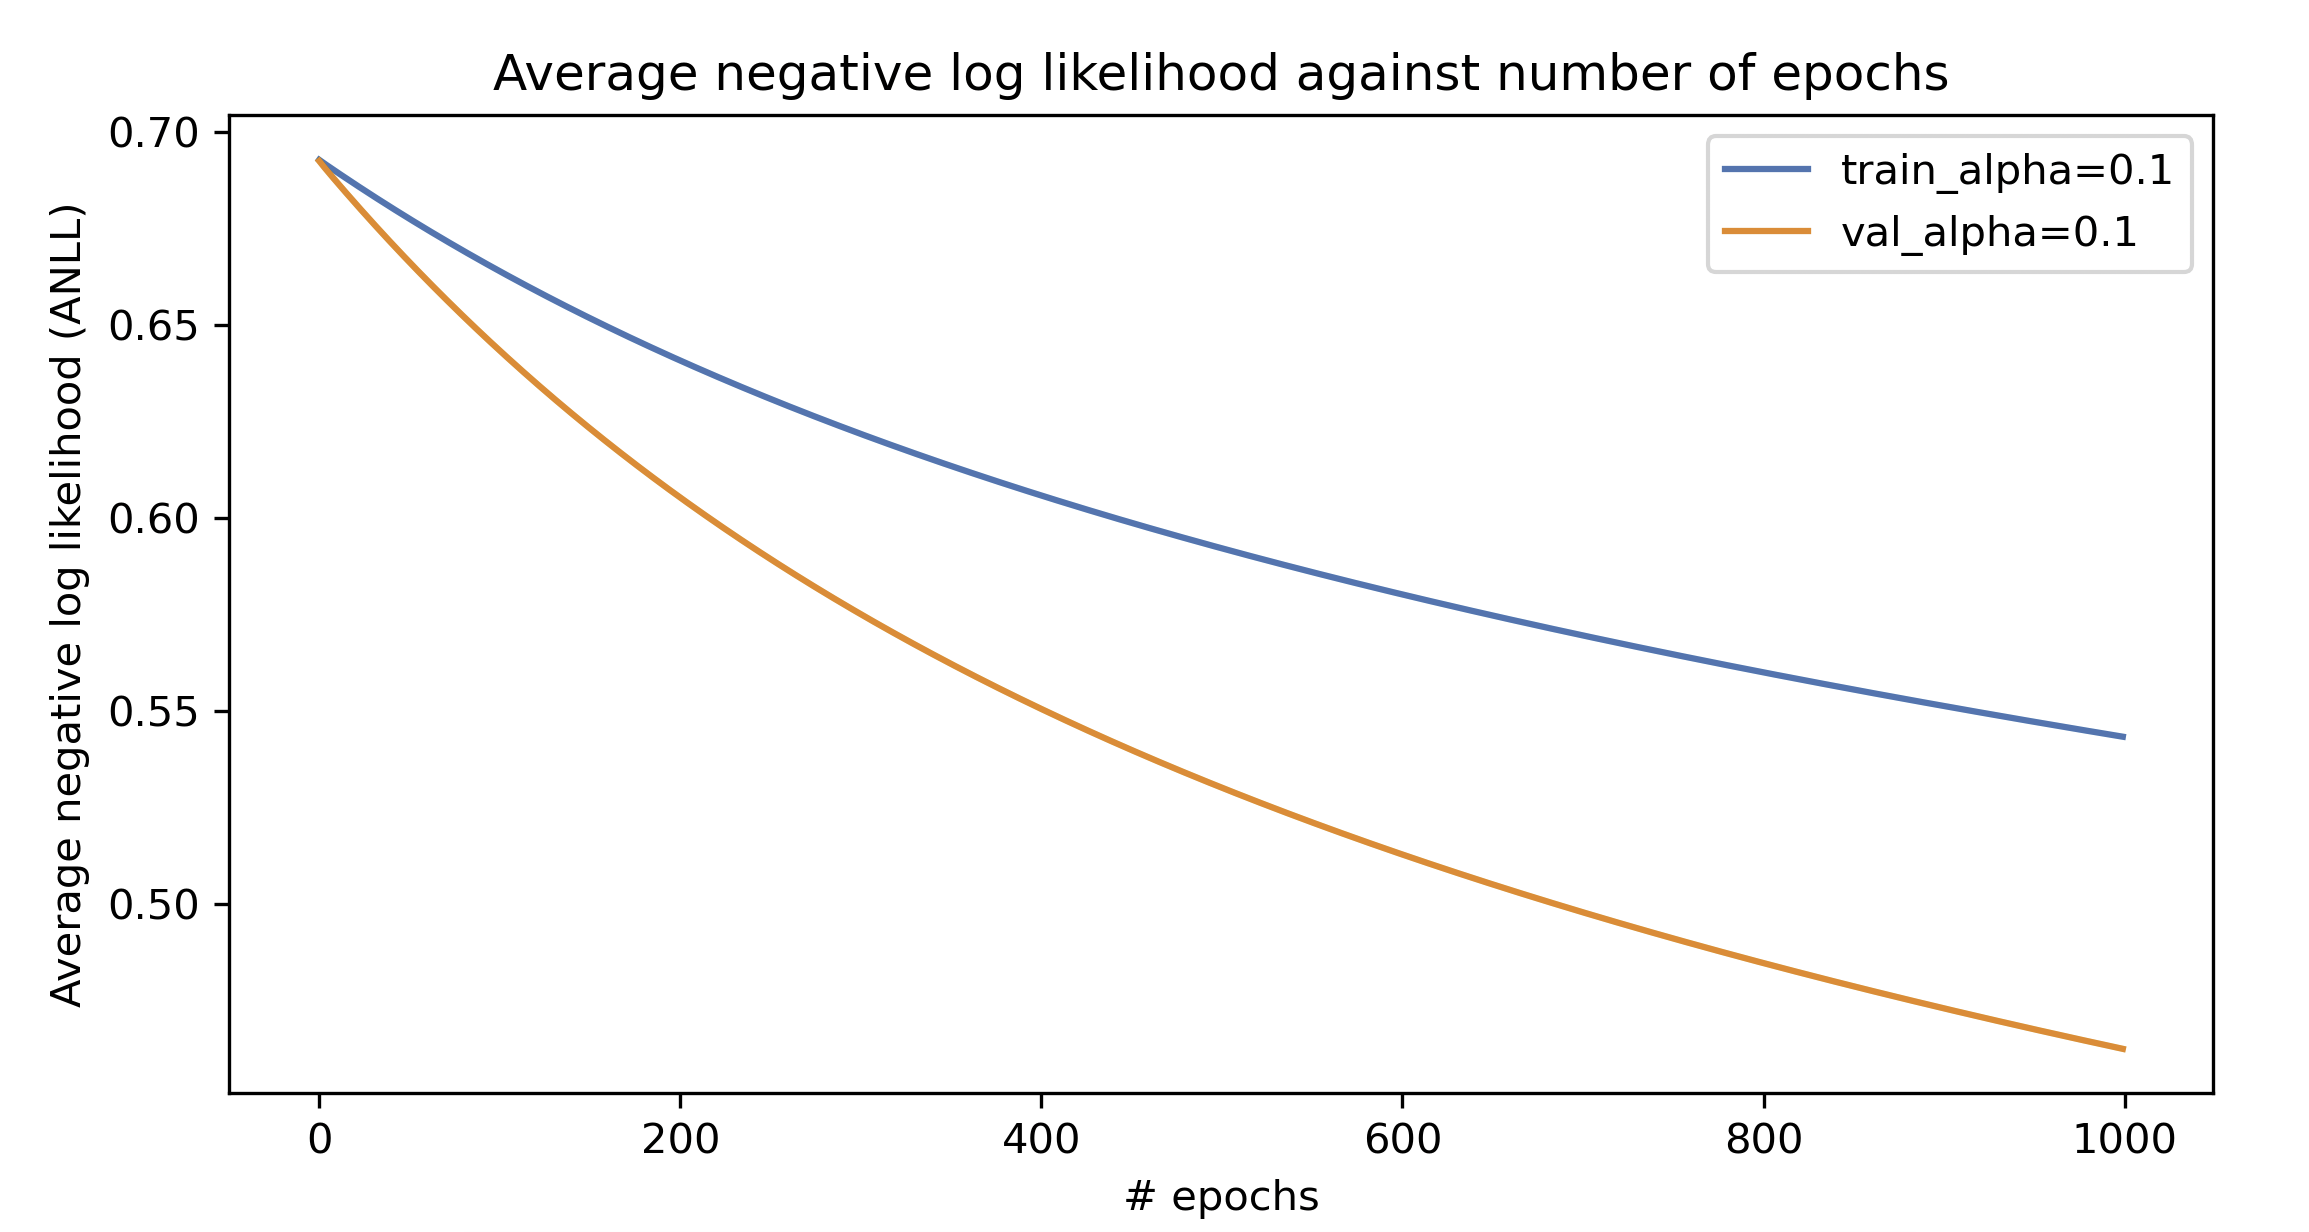
\includegraphics[width = 0.7\textwidth]{1.png}
% YOUR ANSWER 

\begin{center}
% Here is an example of how to include an image:
% \includegraphics{IMAGE FILE PATH HERE}
\end{center}
\end{your_solution}
    


\part[2]
Write a few sentences explaining the output of the above experiment. In particular, do the training and validation log-likelihood curves look the same, or different? Why? 

\begin{your_solution}[height=4cm]
The training and validation log-likelihood curves have a similar shape, but the validation curve consistently has a higher negative log-likelihood value than the training curve. This suggests that the model is overfitting to the training data, as it is not generalizing well to the validation data. This is a common issue in machine learning, and can be addressed through techniques such as regularization or adjusting the model architecture.
% YOUR ANSWER 
\end{your_solution}

\part[2]
Report your train and test error for the large data set (found in the \texttt{largedata} folder in the handout) after running for 1,000 epochs. Please round to the fourth decimal place, e.g., 0.1234.

\begin{your_solution}[width=4cm, height=2cm, title=Train Error]
0.0000
\end{your_solution}
\begin{your_solution}[width=4cm, height=2cm, title=Test Error]
0.1375
\end{your_solution}


\newpage
\part[2]
Using the data in the \texttt{largedata} folder of the handout, make a plot comparing the \emph{training} average negative log-likelihood over epochs for three different values for the learning rates, $\eta \in \{10^{-1}, 10^{-2}, 10^{-3}\}$. The $y$-axis should show the \emph{average} negative log-likelihood, the $x$-axis should show the number of epochs (from 0 to 1,000 epochs), and the plot should contain three curves corresponding to the three values of $\eta$. Provide a legend that indicates the learning rate $\eta$ for each curve.
        
\begin{your_solution}[height=9cm]
% YOUR ANSWER 
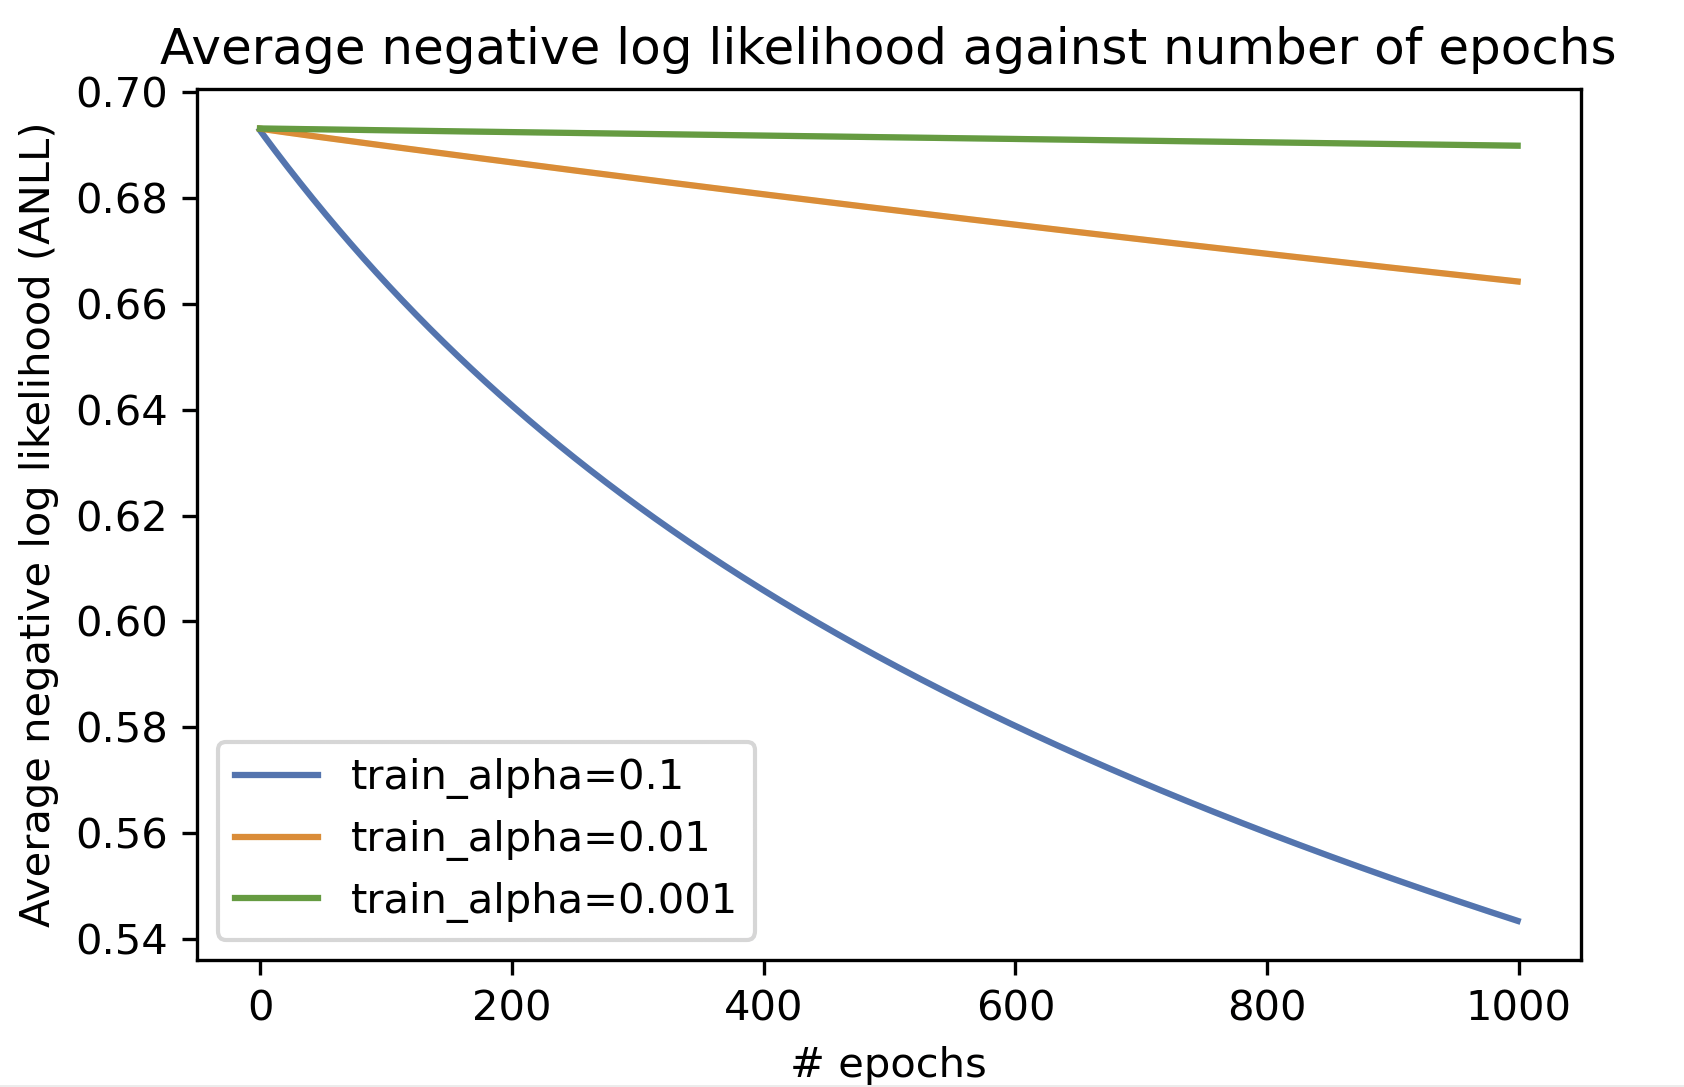
\includegraphics[width = 0.9\textwidth]{2.png}
\begin{center}
% Here is an example of how to include an image:
% \includegraphics{IMAGE FILE PATH HERE}
\end{center}
\end{your_solution}

\part[1] Compare how quickly each curve in the previous question converges.

\begin{your_solution}[height=8cm]
% YOUR ANSWER
Significant, convergence speed:\\
$Learning rate = 0.1 > Learning rate = 0.01 > Learning rate = 0.001$
\end{your_solution}

\end{parts}\newpage
\newpage
\section{Collaboration Questions}
After you have completed all other components of this assignment, report your answers to these questions regarding the collaboration policy. Details of the policy can be found \href{http://www.cs.cmu.edu/~mgormley/courses/10601/syllabus.html}{here}.
\begin{enumerate}
    \item Did you receive any help whatsoever from anyone in solving this assignment? If so, include full details.
    \item Did you give any help whatsoever to anyone in solving this assignment? If so, include full details.
    \item Did you find or come across code that implements any part of this assignment? If so, include full details.
\end{enumerate}

\begin{your_solution}[height=6cm]
% YOUR ANSWER 
1. No
2. No
3. No

\end{your_solution}
\newpage
\end{questions}
\section{Programming (75 points)}

Your goal in this assignment is to implement a working Natural Language Processing (NLP) system using binary logistic regression. Your algorithm will determine whether a restaurant review is positive or negative.

\textbf{Note}: Before starting the programming, you should work through the written component to get a good understanding of important concepts that are useful for this programming component.



\subsection{The Task}\label{task}

{\bf Datasets } 
Download the zip file from the course website, which contains the data for this assignment. This data comes from the Yelp dataset.\footnote{For more details, see \url{https://www.yelp.com/dataset}.} In the data files, each line is a single example that consists of a label (0 for negative reviews and 1 for positive ones) and a set of words. The format of each example (each line) is \lstinline{label\tword1 word2 word3 ... wordN\n}, where words are separated from each other with white-space and the label is separated from the words with a tab character.

Examples of the data are as follows:
 
\begin{lstlisting}
1   i will never forget this single breakfast experience in mad... 
0   the search for decent chinese takeout in madison continues ...
0   sorry but me julio fell way below the standard even for med...
1   so this is the kind of food that will kill you so there s t...
\end{lstlisting}

{\bf Feature Engineering } 
In lecture, we saw that we can apply logistic regression to real-valued inputs of fixed length (e.g. $\xv^{(i)}\in\mathbb{R}^n$). However, each review has variable length and is not real-valued.

To be able to run logistic regression on the dataset, we first need to transform it using some basic feature engineering techniques. In this homework, we will use a word embeddings model, described in full detail in the next section (\ref{featuremodels}).

{\bf Programs } 
At a high level, you will write two programs for this homework: \texttt{feature.py} and \texttt{lr.py}. \texttt{feature.py} takes in the raw input data and produces a real-valued vector for each training, validation, and test example. \texttt{lr.py} then takes in these vectors and trains a logistic regression model to predict whether each example is a positive or negative review.


\subsection{Feature Model}\label{featuremodels}
In order to transform a set of words into vectors, we rely on a popular method of feature engineering: word embeddings.

We use $\boldsymbol{\phi}$ to denote a feature engineering method and $\xv^{(i)}$ to denote a training example (a set of English words as seen in \ref{task}).

Rather than simply indicating which words are present, word embeddings represent each word by ``embedding'' it into a low-dimensional vector space, which may carry more information about the semantic meaning of the word. In this homework, we use the \emph{GloVe} embeddings, a commonly used set of feature vectors. \footnote{For more details on how these embeddings were trained, see the original work at   \url{https://nlp.stanford.edu/projects/glove/}}

{\bf Embeddings }
\texttt{glove\_embeddings.txt} contains the \emph{GloVe} embeddings of \texttt{6792} words. 
Not every word in each review is present in the provided \texttt{glove\_embeddings.txt} file. We treat such missing words as ``out-of-vocabulary'' and ignore them. Each line consists of a word and its embedding separated by tabs:

\lstinline{word\tfeature1\tfeature2\t...feature300\n}. Each word's embedding is always a 300-dimensional vector. As an example, here are the first few lines of \texttt{glove\_embeddings.txt}, with values rounded to 3 decimal places:
% \begin{lstlisting}
%    comic   -0.119   -1.952   -0.226   -0.825    5.625   -0.266   ...
%    from    -0.114   -2.072   -0.874   -0.483    0.354   -2.205   ...
%    from    -0.114   -2.072   -0.874   -0.483    0.354   -2.205   ...
%    comic   -0.119   -1.952   -0.226   -0.825    5.625   -0.266   ...
% \end{lstlisting}
\begin{lstlisting}
deserves  0.175  -0.153  -0.208  0.092  0.222   0.202  ...
butter    0.357   0.469  -0.021  0.024 -0.168  -0.213 ...
staffing -0.076   0.212  -0.384  0.552 -0.193  -0.052 ...
weird     0.110   0.090   0.139  0.340 -0.098  -0.113 ...     
\end{lstlisting}


{\bf Using Word Embeddings }
For this model, there will be two steps in the feature engineering process: 
    
\begin{enumerate}
    \item First, we would like to exclude words from the review that are not included in the  \emph{GloVe} dictionary. Let  $\xv\_\text{trim}^{(i)} = \text{TRIM}(\xv^{(i)})$, where $\text{TRIM}(\xv^{(i)})$ trims the list of words $\xv^{(i)}$ by only including words of $\xv^{(i)}$ present in \texttt{glove\_embeddings.txt}.
    \item Second, we want to take the trimmed vector $\xv\_\text{trim}^{(i)}$ and convert it to the final feature vector by averaging the  \emph{GloVe} embeddings of its words:
    $$\boldsymbol{\phi}\left(\xv^{(i)}\right) = \frac{1}{J} \sum_{j=1}^J \emph{GloVe}(\xv\_\text{trim}^{(i)}_j) $$
    where $J$ denotes the number of words in $\xv\_\text{trim}^{(i)}$ and $\xv\_\text{trim}^{(i)}_j$ is the j-th word in $\xv\_\text{trim}^{(i)}$.
    
     In the given equation, $\emph{GloVe}(\xv\_\text{trim}^{(i)}_j) \in \mathbb{R}^{300}$ is the \emph{GloVe} feature vector for the word $\xv\_\text{trim}^{(i)}_j$.
\end{enumerate}
    
The following \textbf{example} provides a reference:

\begin{itemize}
    \item Let $\xv^{(i)}$ denote the sentence ``\texttt{a hot dog is not a sandwich because it is not\\ square}''.
    \item A toy \emph{GloVe} dictionary is given as follows: 
    \begin{lstlisting}
hot         0.1    0.2    0.3
not        -0.1    0.2   -0.3
sandwich    0.0   -0.2    0.4
square      0.2   -0.1    0.5
    \end{lstlisting}
    \item Then, $\xv\_\text{trim}^{(i)}$ denotes the trimmed review ``\texttt{hot not sandwich not square}''. In this trimmed text, the words that are not in the \emph{GloVe} dictionary are excluded. Also note that we keep the order of words and do not de-duplicate words in the trimmed text. \footnote{Keeping duplicates is equivalent to weighting words by their frequency. If \lstinline{"good"} appears 3 times as often as \lstinline{"bad"}, the movie review is more likely to be positive than negative.}
    \item The feature for $\xv^{(i)}$ can be calculated as
        \begin{align*} \boldsymbol{\phi}_2(\xv^{(i)}) &= \frac{1}{5}\big( \emph{GloVe}(\text{hot}) + 2 \cdot \emph{GloVe}(\text{not}) + \emph{GloVe}(\text{sandwich}) + \emph{GloVe}(\text{square}) \big) \\
        &= \begin{bmatrix} 0.02 & 0.06 & 0.12 \end{bmatrix}^T.
        \end{align*}
\end{itemize}

\subsection{\texttt{feature.py}}\label{featurepy}

\lstinline{feature.py} implements word embeddings (described above in \ref{featuremodels}) to transform raw training examples (a label and a list of English words) to formatted training examples (a label and a feature vector).

{\bf Inputs }
\begin{itemize}
    \item \textbf{Input data} for training, validation, and testing. Each data point contains a label and an English restaurant review in the format described in \ref{task}.
    \item \textbf{\emph{GloVe} embeddings} to use for the word embedding feature extraction methods.
\end{itemize}

{\bf Outputs }
\begin{itemize}
    \item \textbf{Formatted data} for training, validation, and testing. You should perform feature extraction on \textit{each} of the training, validation, and test sets.
\end{itemize}

{\bf Output Format }
Each output file (one for training data, one for validation, and one for testing) should contain the formatted presentation of each example printed on a new line. Use \lstinline{\n} to create a new line. The format for each line should exactly match \lstinline{label\tvalue1\tvalue2\tvalue3\t...valueM\n}.

Each line corresponds to a particular restaurant review, where the first entry is the label and the rest are the features in the feature vector. The rows are the summed up \emph{GloVe} vectors for all the words present in the dictionary. All entries are separated with a tab character. The handout folder contains example formatted outputs on the small dataset; they are partially reproduced below for your reference. Please round your outputs to 6 decimal places.


\begin{lstlisting}
1.000000	-0.166646	 0.641027	-0.064805	...
0.000000	-0.224874	 0.461526	-0.215232	...
0.000000	-0.222178	 0.437475	-0.083073	...
1.000000	-0.215923	 0.612535	 0.061671	...
\end{lstlisting}

\subsection{\texttt{lr.py}}\label{lrpy}

\lstinline{lr.py} implements a logistic regression classifier that takes in formatted training data and produces a label (either 0 or 1) that corresponds to whether each restaurant review was negative or positive.
{\bf Inputs }
\begin{itemize}
    \item \textbf{Formatted data} for training, validation, and testing. Each data point contains a label and a corresponding feature vector. These files are the ones produced by \lstinline{feature.py}.
    \item \textbf{The number of epochs} to train for, which will be passed in as a command line argument.
    \item \textbf{The learning rate}, also passed in via the command line.
\end{itemize}

{\bf Requirements }
\begin{itemize}
    \item Include an intercept term in your model. You can either treat the intercept term as a separate variable, or fold it into the parameter vector (recommended). In either case, make sure you update the intercept parameter correctly.
    \item Initialize all model parameters to 0.
    \item Use stochastic gradient descent (SGD) to train the logistic regression model.
    \item Perform SGD updates on the training data \textbf{in the order that the data is given in the input file}. While we would normally shuffle training examples in SGD, we need training to be deterministic in order to autograde this assignment. \textbf{Do not shuffle the training data.}
\end{itemize}

{\bf Outputs }
\begin{itemize}
    \item \textbf{Labels} for the training and testing data.
    \item \textbf{Metrics} for the training and testing error.
\end{itemize}

{\bf Output Labels Format }
Your \lstinline{lr} program should produce two output \texttt{.txt} files containing the predictions of your model on training data and test data. Each file should contain the predicted labels for each example printed on a new line. The name of these files will be passed as command line arguments. Use \lstinline{\n} to create a new line. An example of the labels is given below.

\begin{lstlisting}
1
0
0
1
\end{lstlisting}

{\bf Output Metrics Format }
Your program should generate a \texttt{.txt} file where you report the final training and testing error after training has completed. The name of this file will be passed as a command line argument.

All of your reported numbers should be within 0.00001 of the reference solution, and you should round the error values to 6 decimal places. The following example is the reference solution for the small dataset after 500 training epochs with learning rate 0.1.
\begin{lstlisting}
error(train): 0.000000
error(test): 0.625000
\end{lstlisting}

Each line in the output file should be terminated by a newline character \lstinline{\n}. There is a whitespace character after the colon.

\begin{figure}[H]
        \centering
        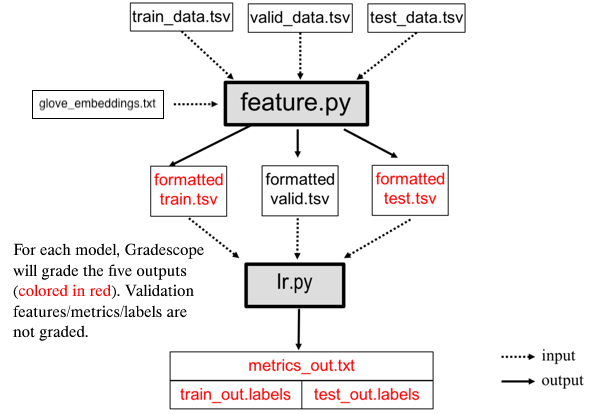
\includegraphics[width = 0.7\textwidth]{fig/Pipeline_v5.png}
        \caption{Programming pipeline for sentiment analyzer based on binary logistic regression}
        \label{pipeline}
\end{figure}

\subsection{Command Line Arguments}\label{commandline}
The autograder runs and evaluates the output from the files generated, using the following command (note \lstinline{feature} will be run before \lstinline{lr}):

\begin{tabbing}
\=\texttt{\$ \textbf{python} feature.\textbf{py} [args1\dots]}\\
\>\texttt{\$ \textbf{python} lr.\textbf{py} [args2\dots]}
\end{tabbing}

Where above \texttt{[args1\dots]} is a placeholder for seven command-line arguments: \texttt{<train\_input>}\newline \texttt{<validation\_input> <test\_input>  <feature\_dictionary\_input> \newline <formatted\_train\_out> <formatted\_validation\_out>  <formatted\_test\_out> }. These arguments are described in detail below:
\begin{enumerate}
    \item \texttt{<train\_input>}: path to the training input \texttt{.tsv} file (see Section~\ref{task})
    \item \texttt{<validation\_input>}: path to the validation input \texttt{.tsv} file (see Section~\ref{task})
    \item \texttt{<test\_input>}: path to the test input \texttt{.tsv} file (see Section~\ref{task})
    \item \texttt{<feature\_dictionary\_input>}: path to the \emph{GloVe} feature dictionary \texttt{.txt} file (see Section~\ref{featuremodels})
    \item \texttt{<formatted\_train\_out>}: path to output \texttt{.tsv} file to which the feature extractions on the \emph{training} data should be written (see Section~\ref{featurepy})
    \item \texttt{<formatted\_validation\_out>}: path to output \texttt{.tsv} file to which the feature extractions on the \emph{validation} data should be written (see Section~\ref{featurepy})
    \item \texttt{<formatted\_test\_out>}: path to output \texttt{.tsv} file to which the feature extractions on the \emph{test} data should be written (see Section~\ref{featurepy})
\end{enumerate}


Likewise, \texttt{[args2\dots]} is a placeholder for eight command-line arguments: \texttt{<formatted\_train\_input>} \texttt{<formatted\_validation\_input> <formatted\_test\_input> <train\_out> <test\_out> <metrics\_out> <num\_epoch> <learning\_rate>}. These arguments are described in detail below:
\begin{enumerate}
    \item \texttt{<formatted\_train\_input>}: path to the formatted training input \texttt{.tsv} file (see Section~\ref{featurepy})
    \item \texttt{<formatted\_validation\_input>}: path to the formatted validation input \texttt{.tsv} file (see Section~\ref{featurepy})
    \item \texttt{<formatted\_test\_input>}: path to the formatted test input \texttt{.tsv} file (see Section~\ref{featurepy})
    \item \texttt{<train\_out>}: path to output \texttt{.txt} file to which the prediction on the \emph{training} data should be written (see Section~\ref{lrpy})
    \item \texttt{<test\_out>}: path to output \texttt{.txt} file to which the prediction on the \emph{test} data should be written (see Section~\ref{lrpy})
    \item \texttt{<metrics\_out>}: path of the output \texttt{.txt} file to which metrics such as train and test error should be written (see Section~\ref{lrpy})
    \item \texttt{<num\_epoch>}: integer specifying the number of times SGD loops through all of the training data (e.g., if \texttt{<num\_epoch>} equals 5, then each training example will be used in SGD 5 times). 
    \item \texttt{<learning\_rate>}: float specifying the learning rate; in the reference output, we set the learning rate to be $0.1$ for all datasets
\end{enumerate}

As an example, the following two command lines would run your programs on the large dataset in the handout for 500 epochs. You are given the output of this command and the equivalent command on the small dataset in the handout directories \verb|largeoutput| and \verb|smalloutput|.

\begin{lstlisting}[language=Shell]
$ python feature.py \ 
largedata/train_large.tsv \
largedata/val_large.tsv \
largedata/test_large.tsv \
glove_embeddings.txt \
largeoutput/formatted_train_large.tsv \
largeoutput/formatted_val_large.tsv \
largeoutput/formatted_test_large.tsv

$ python lr.py \
largeoutput/formatted_train_large.tsv \
largeoutput/formatted_val_large.tsv \
largeoutput/formatted_test_large.tsv \
largeoutput/formatted_train_labels.txt \
largeoutput/formatted_test_labels.txt \
largeoutput/formatted_metrics.txt \
500 \
0.1
\end{lstlisting}

\begin{notebox}
{\bf Important Note:} You will not be writing out the predictions on validation data, only on train and test data. The validation data is \emph{only} used to give you an estimate of held-out negative log-likelihood at the end of each epoch during training. You are asked to graph the negative log-likelihood vs. epoch of the validation and training data in Programming Empirical Questions section. \footnote{For this assignment, we will always specify the number of epochs. However, a more mature implementation would monitor the performance on validation data at the end of each epoch and stop SGD when this validation log-likelihood appears to have converged. You should \textbf{\emph{not}} implement such a convergence check for this assignment.} 
\end{notebox}


\subsection{Starter Code}\label{startercode}

To help you start this assignment, we have provided starter code in the handout.



\subsection{Gradescope Submission }
You should submit your \texttt{feature.py} and \texttt{lr.py} to Gradescope.
\textit{Note}: please do not zip them or use other file names. This will cause problems for the autograder to correctly detect and run your code. Gradescope will also provide \textbf{hints for common bugs}; Ctrl-F for HINT if you did not receive a full score.

\end{document}